\documentclass[11pt]{article}
\usepackage[a4paper,margin=24mm]{geometry}
\usepackage{amsmath,amssymb,booktabs,array,graphicx,microtype}
\usepackage{xcolor,tikz,xurl}
\usepackage{placeins}
\usetikzlibrary{arrows.meta,positioning,fit,calc}
\usepackage[colorlinks=true,linkcolor=blue!50!black,citecolor=blue!50!black,urlcolor=blue!50!black]{hyperref}
\newcommand{\id}{\mathbb I}
\newcommand{\tr}{\operatorname{tr}}
\newcommand{\tS}{\widetilde S}
\newcommand{\Dg}{D_{\mathrm{grow}}}
\newcommand{\Gz}{G_{\mathrm{bare}}}
\newcommand{\Gt}{G_{\mathrm{grow}}}
\newcommand{\code}[1]{{\small\nolinkurl{#1}}}
\newcommand{\norm}[1]{\left\lVert#1\right\rVert}
\newcommand{\smallnote}[1]{\par\smallskip\noindent\textit{#1}\par\smallskip}
\tikzset{m/.style={draw=blue!65!black,fill=blue!7,minimum width=10mm,minimum height=7mm},
 a/.style={draw=green!40!black,fill=green!8,minimum width=10mm,minimum height=7mm},
 r/.style={draw=orange!70!black,fill=orange!8,minimum width=10mm,minimum height=7mm},
 g/.style={draw=purple!70!black,fill=purple!6,minimum width=14mm,minimum height=8mm},
 flow/.style={-{Latex},thick},wire/.style={thick},txt/.style={align=center,font=\small}}
\title{Boundary MPS, L-shaped environments, and six-$R$ replica contractions\\
\large RK--Ising and the square-lattice transverse-field Ising model\\
\ifdetailed Detailed methods and verification notes\else Concise methods guide\fi}
\author{Project methods note}
\date{17 September 2026}
\begin{document}
\maketitle
\begin{abstract}
We specify the route from a two-dimensional tensor-network state to a boundary MPS,
an L-shaped boundary representation (LMPS), and the tripartite replica observable
$\tS$. The RK--Ising wavefunction is constructed analytically; the TFIM PEPS is
prepared by variational optimization with a CTMRG environment, after which VUMPS
is used for its boundary transfer problem. We distinguish a bare two-column
overlap, a three-column transfer contraction, and the metric formed from grown
half-chain environments. These objects are not interchangeable by definition.
The six-$R$ stage is specified by replica permutations, endpoint ownership, and
normalization. Mathematical identities are separated from finite-bond
approximations and numerical checks. In particular, agreement between two
implementations is not a general proof of endpoint factorization.
\end{abstract}
\ifdetailed\setcounter{tocdepth}{2}\tableofcontents\newpage\fi

\section{Scope, geometry, and notation}
Regions $A$ and $B$ occupy the upper-left and upper-right quadrants; $C$ is the
lower half-plane. $AB$ is a vertical seam and $AC,BC$ are horizontal seams.
The LMPS describes two rays and their junction, not just a straight boundary
tensor with its indices relabelled. An oriented rail is a local tensor used
repeatedly on a particular ray. Endpoint, rail, and replica endpoint are
different objects.

\begin{center}
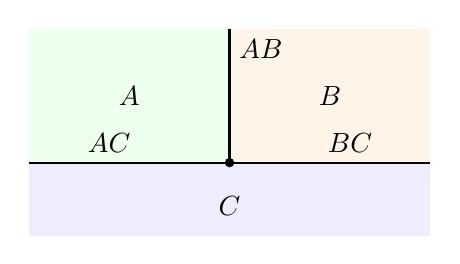
\begin{tikzpicture}[scale=.85]
\fill[green!7] (-3,0) rectangle (0,2);
\fill[orange!9] (0,0) rectangle (3,2);
\fill[blue!7] (-3,-1.1) rectangle (3,0);
\draw[thick] (-3,0)--(3,0);\draw[thick] (0,0)--(0,2);
\node at (-1.5,1){$A$};\node at (1.5,1){$B$};\node at (0,-.65){$C$};
\node[above] at (-1.8,0){$AC$};\node[above] at (1.8,0){$BC$};
\node[right] at (0,1.7){$AB$};\fill (0,0) circle(2pt);
\end{tikzpicture}
\end{center}

\begin{center}\small
\begin{tabular}{p{28mm}p{116mm}}
\toprule
Symbol & Meaning\\\midrule
$A^s$ & Local PEPS tensor; $s$ is the physical spin. Region $A$ is distinguished by context.\\
$D$ & PEPS virtual bond dimension, a variational-state parameter.\\
$\chi_{\rm CTM}$ & Environment dimension used in the TFIM energy/gradient calculation.\\
$\chi$ & Boundary-MPS bond dimension used for fixed-state measurements.\\
$a_{nwse}$ & One norm-transfer tensor, with explicitly ordered north, west, south, east legs.\\
$T$ & A complete row or column of repeated $a$ tensors; direction is stated explicitly.\\
$M_L^p,M_R^p$ & Local tensors on the spatial sides of a ladder; not whole half-infinite maps.\\
$A_L^p,A_R^p,C$ & Canonical tensors and center matrix of one boundary MPS.\\
$\Dg^p$ & One local boundary tensor after absorption of one $a$.\\
$L_n^{(g)},R_n^{(g)}$ & Finite-depth mixed grown-tail contractions.\\
$K_{XY}$ & One-copy mixed seam fixed point between the incident regional rails.\\
$\mathcal R_{XY,ij}$ & Rank-four two-cycle replica endpoint; six such objects close $Z_4$.\\
\bottomrule
\end{tabular}
\end{center}
All logarithms are natural. A superscript $p$ selects a local boundary physical
index, not the physical TFIM spin $s$. In the uncompressed quantum norm layer,
$p=(k,b)$ has dimension $d_{\rm eff}=D^2$. A dagger denotes a bra contraction;
ordinary spatial tensor contractions do not acquire a dagger merely because
a tensor is called ``left'' or ``right''.

\section{Input states and ground-state preparation}
\subsection{RK--Ising: an explicitly known state}
With Ising spins $s_i=\pm1$, coupling set to one, and
$E(s)=-\sum_{\langle ij\rangle}s_i s_j$, define
\begin{equation}
 |\Psi_\beta\rangle=Z(\beta)^{-1/2}
 \sum_s e^{-\beta E(s)/2}|s\rangle,
 \qquad Z(\beta)=\sum_s e^{-\beta E(s)}.
\end{equation}
There is no variational GS optimization in this benchmark. Set
$W_{1/2}(s,t)=e^{\beta st/2}$ and factor the positive matrix
$W_{1/2}=Q Q^{\mathsf T}$. A real symmetric square root is convenient. Then
\begin{equation}
 A^s_{uldr}=Q_{su}Q_{sl}Q_{sd}Q_{sr}
\end{equation}
is an exact $D=2$ representation of the unnormalized amplitudes.
The half in the Boltzmann exponent is \emph{elementwise}; taking a matrix
fourth root of the full Boltzmann matrix is not the same operation.
The norm must reproduce the classical partition function. This provides
an absolute free-energy benchmark for tensor normalization and contraction.

\subsection{TFIM: variational PEPS followed by boundary VUMPS}
Our convention uses Pauli matrices with eigenvalues $\pm1$:
\begin{equation}
 H=-J\sum_{\langle ij\rangle}\sigma_i^z\sigma_j^z
   -h\sum_i\sigma_i^x,\qquad J=1.
\end{equation}
The finite-$D$ state is found by minimizing the energy per site
$e(A)=\langle\Psi(A)|H|\Psi(A)\rangle/
\langle\Psi(A)|\Psi(A)\rangle$ with the extensive normalization understood.
In the current production workflow the environment and AD gradient are
computed using CTMRG~\cite{ctm}, followed by a gradient-based PEPS update.
Random initial tensors and simple-update initial states are supported.
Simple update is an initializer, not an independent certification of
variational optimality. Ordered/disordered run labels describe initializations
or continuation histories; the final magnetization determines the observed
symmetry breaking. Differentiable tensor-network optimization is described
in Ref.~\cite{liao}.

\smallnote{VUMPS is not the TFIM PEPS GS optimizer in these runs. It solves the
boundary of the saved GS candidate. In a one-dimensional Hamiltonian problem
VUMPS can itself optimize a ground-state MPS; that is a different application.}

\ifdetailed
\subsection{What must be saved and checked}
Store the PEPS, CTMRG environment, Hamiltonian convention, symmetry constraints,
initialization, continuation parent, optimizer iteration, energy, and projected
gradient. Save accepted optimizer steps atomically, so a preempted job can
resume without inventing a new source state. A tensor selected for entropy
measurements must be pinned by its byte-level hash; a mutable ``selected''
alias is not sufficient provenance.

For the C4v-constrained runs, gradients are evaluated in the allowed tangent
space. A large unprojected gradient does not by itself disprove convergence
inside that constrained family. Conversely a small projected gradient does
not exclude a lower-energy state outside the family. Fresh CTMRG environments
and independent contraction implementations test the gradient on the same
saved tensor. Compare energies between branches at compatible environment
accuracy; select neither a state nor a random seed because its entropy curve
looks smoother. Near an unresolved crossing retain both candidates.

\subsection{Spatial symmetry is a checked input, not a model-name shortcut}
An isotropic Hamiltonian permits a C4v ansatz but does not force an arbitrary
numerical PEPS tensor to have C4v symmetry. Check the implemented tensor
constraint, the norm transfer under rotations/reflections, the bond-space
orientations, and the chosen boundary sector before reusing a boundary.
RK--Ising admits a symmetric fast path. General quantum tensors require
directional/regional boundaries and mixed seam maps. Internal Ising $\mathbb Z_2$
symmetry, spatial C4v symmetry, and boundary-MPS gauge freedom are distinct.
For complex tensors, distinguish a spatial reflection from a reflection
combined with complex conjugation. In the installed PEPSKit implementation,
the one-site \code{RotateReflect} projection uses a conjugating reflection
(\code{herm\_depth}), not just an index permutation. A saved TFIM tensor
can therefore satisfy this constraint without satisfying plain reflection
in its stored bond coordinates. Reusing directional boundaries requires
carrying the actual transformations, including any conjugation and virtual
basis changes; the name of the projection alone does not justify identical
arrays on all rails.
The current quantum six-$R$ bridge is a one-site, uniform-virtual-dimension
implementation; arbitrary multi-site cells require a multiline boundary and
consistent blocking, not a relabelled one-site formula.
\fi

\section{Norm transfer and the VUMPS boundary}
In the quantum layer, contract the physical spin exactly once:
\begin{equation}
 a_{(n,n')(w,w')(s,s')(e,e')}=
 \sum_\sigma A^\sigma_{n e s w}\,
              \overline{A^\sigma_{n'e's'w'}}.
\end{equation}
Here the PEPS axes are $(\sigma,N,E,S,W)$ whereas $a$ is stored as $(N,W,S,E)$.
Fuse each ket/bra pair in a fixed order, e.g. $k+D(b-1)$. Preserve the physical
ket/bra factors until replica wiring; a dense reshape cannot silently replace
the dual-space maps of a typed tensor library.

VUMPS approximates a dominant boundary of the infinite transfer operator,
\begin{equation}
 T|M\rangle\simeq\Lambda |M\rangle,
 \qquad A_C^p=A_L^p C=C A_R^p,
\end{equation}
with the canonical conditions
\begin{equation}\label{eq:canonical}
 \sum_p(A_L^p)^\dagger A_L^p=\id,
 \qquad\sum_p A_R^p(A_R^p)^\dagger=\id.
\end{equation}
References~\cite{vumps,schollwock} provide the variational and canonical MPS
framework. These references are not a proof of this project's endpoint
replacement. In a non-Hermitian transfer problem one must retain the actual
left/right environments and test their eigen-residuals, not assume that a
Hermitian energy operator makes every spatial transfer matrix Hermitian.

\ifdetailed
\subsection{The gauge actually returned and used: one boundary at a time}
Write $q\in\{N,E,S,W\}$ for a spatial side, and reserve $C_q$ for its
\emph{center matrix}, not region $C$. One VUMPS solve returns
$(A_{L,q},A_{R,q},A_{C,q},C_q)$ in mixed canonical form. Here the subscripts
$L,R$ on $A$ label canonical descriptions of \emph{one state}; they do not
label the west and east sides of the PEPS. In local chain coordinates,
\begin{equation}
 |M_q\rangle=\cdots A_{L,q}A_{L,q}\,C_q\,A_{R,q}A_{R,q}\cdots,
 \qquad A_{L,q}^p C_q=C_q A_{R,q}^p=A_{C,q}^p.
\end{equation}
The equality is exact for an exact canonical representation and is checked
up to the stored center residual in a numerical solve. The center can be
moved through a site using this identity; it cannot simply be deleted.

\begin{figure}[htbp]\centering
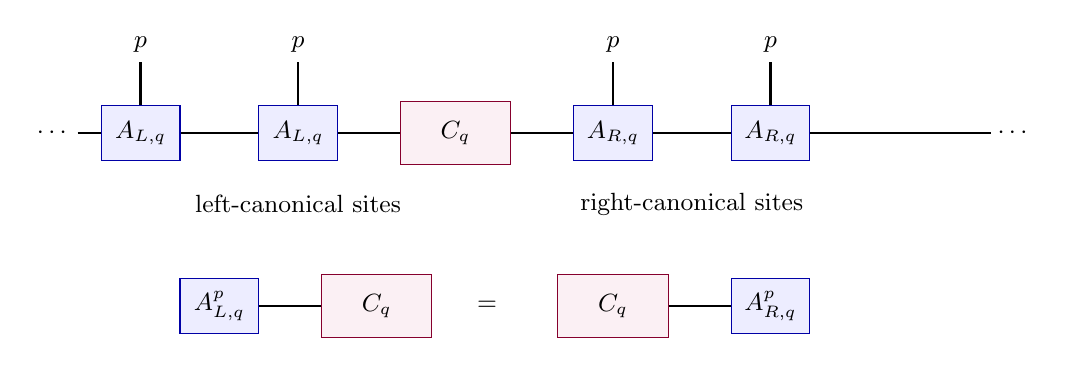
\begin{tikzpicture}[x=1cm,y=1cm,font=\small]
\draw[wire](-.8,0)--(10.8,0);
\foreach \x/\lab in {0/{A_{L,q}},2/{A_{L,q}},6/{A_{R,q}},8/{A_{R,q}}}{
 \node[m] at (\x,0){$\lab$};\draw[wire](\x,.36)--(\x,.9);
 \node[above] at (\x,.9){$p$};}
\node[g] at (4,0){$C_q$};
\node at (-1.1,0){$\cdots$};\node at (11.1,0){$\cdots$};
\node[txt] at (2,-.9){left-canonical sites};
\node[txt] at (7,-.9){right-canonical sites};
\node[m](al) at (1,-2.2){$A_{L,q}^p$};\node[g](cl) at (3,-2.2){$C_q$};
\draw[wire](al)--(cl);\node at (4.4,-2.2){$=$};
\node[g](cr) at (6,-2.2){$C_q$};\node[m](ar) at (8,-2.2){$A_{R,q}^p$};
\draw[wire](cr)--(ar);
\end{tikzpicture}
\caption{One boundary, two canonical charts. Physical legs are open. The
center connects the charts; it is not a spatial corner or a mixed-seam metric.}
\end{figure}

The bare cardinal driver exports \code{boundary.state.AL[1]} on \emph{each}
side. It does not export $A_L$ for the west side and $A_R$ for the east side.
The raw tensor on each rotated side is thus left canonical in that solve's
own chain direction. The south and west exports then exchange the two bond
axes to restore global orientation, as listed in Section~4.1. Such a reflected
array need not remain left canonical in the new array ordering.
For example, with $\widehat M^p=(A_L^p)^{\mathsf T}$,
\begin{equation}
 \sum_p\widehat M^p(\widehat M^p)^\dagger
 =\left[\sum_p(A_L^p)^\dagger A_L^p\right]^{\mathsf T}=\id.
\end{equation}
It is right canonical in that ordering, but is \emph{not thereby the stored}
$A_R$ of the same solve. This is spatial bond reversal, not the gauge change
implemented by $C_q$.

\paragraph{What is not jointly canonicalized.}
The driver keeps the numerical bond bases returned by the separate solves;
it does not jointly gauge-fix west against east, or region $A$ against region
$B$. Within one boundary, a compatible change of canonical charts has
$A_L^p\mapsto U^\dagger A_L^pU$, $A_R^p\mapsto V^\dagger A_R^pV$,
$C\mapsto U^\dagger CV$ for unitary $U,V$. The canonical conditions survive.
Thus canonicality alone does not identify independently obtained bases.
The term \emph{common chart} below refers to explicit center/metric transport
inside one constructed regional object, not to a demonstrated joint canonical
gauge for all boundaries. No diagonal, positive $C_q$ convention is assumed
unless the saved arrays have actually been transformed to that convention.

\paragraph{Which infinite self-contraction is identity?}
For left-canonical sites, propagate from the left using
$X\mapsto\sum_p(A_L^p)^\dagger X A_L^p$; for right-canonical sites,
propagate from the right using $Y\mapsto\sum_p A_R^pY(A_R^p)^\dagger$.
Identity is a fixed point of these two \emph{bra--ket} channels.
Convergence to it from arbitrary far caps additionally needs the relevant
mixing/sector assumptions. It is not the value of an arbitrary bilinear
spatial ladder without the indicated complex conjugations.

\begin{figure}[htbp]\centering
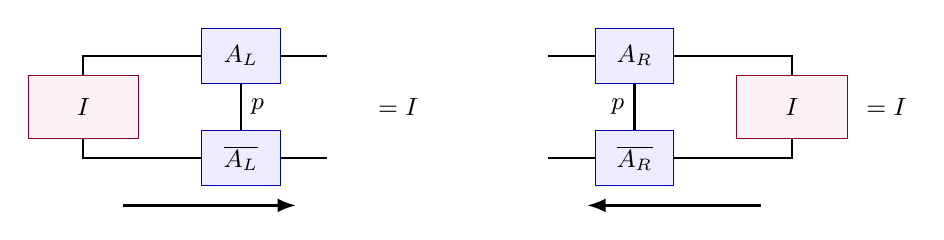
\begin{tikzpicture}[x=1cm,y=1cm,font=\small]
\node[g](il) at (0,0){$I$};
\node[m](ak) at (2,.65){$A_L$};\node[m](ab) at (2,-.65){$\overline{A_L}$};
\draw[wire](il.north)--(0,.65)--(ak);\draw[wire](il.south)--(0,-.65)--(ab);
\draw[wire](ak)--node[right]{$p$}(ab);
\draw[wire](ak.east)--(3.1,.65);\draw[wire](ab.east)--(3.1,-.65);
\node at (4,0){$=I$};\draw[flow](.5,-1.25)--(2.7,-1.25);
\node[m](rk) at (7,.65){$A_R$};\node[m](rb) at (7,-.65){$\overline{A_R}$};
\node[g](ir) at (9,0){$I$};
\draw[wire](rk)--node[left]{$p$}(rb);
\draw[wire](rk.east)--(9,.65)--(ir.north);
\draw[wire](rb.east)--(9,-.65)--(ir.south);
\draw[wire](rk.west)--(5.9,.65);\draw[wire](rb.west)--(5.9,-.65);
\node at (10.2,0){$=I$};\draw[flow](8.6,-1.25)--(6.4,-1.25);
\end{tikzpicture}
\caption{The two canonical identity contractions. Arrows indicate propagation
along the chain, not geographical north/south. The bar is essential.}
\end{figure}

\subsection{Iteration and stopping conditions}
Initialize a boundary MPS in the transfer's actual physical space. In each
VUMPS step, construct the left/right transfer environments, solve the effective
center-tensor and center-matrix problems, and restore a consistent mixed
canonical representation. Stop only after the variational (Galerkin),
environment, and center-consistency residuals meet the recorded tolerances.
For an eigenproblem $\mathcal E(X)=\lambda X$ use, for example,
\begin{equation}
 r_X=\frac{\norm{\mathcal E(X)-\lambda X}}
 {\max(\norm{\mathcal E(X)},|\lambda|\norm X,\epsilon)}.
\end{equation}
Near degeneracy, several low-residual boundary candidates can be distinct.
Record all attempted seeds, convergence flags, row eigenvalues, magnetizations,
and the selection rule. Historical drivers differ: some selected the first
converged candidate; others selected the largest row-eigenvalue magnitude among
converged trials. This difference can precede, and contaminate, any direct/endmap
comparison. Matching candidate-selection criteria is not the same as sharing
the two methods' boundary checkpoint.

\subsection{Which contraction gives identity?}
Equation~\eqref{eq:canonical} makes identity a fixed point of the \emph{specified
self-overlap channel in the specified direction}. It does not state that
every spatial $M_L|M_R$ ladder or every $K_{XY}$ equals identity. The relation
$A_L^p C=C A_R^p$ concerns two canonical descriptions of the same MPS and its
center matrix. A general mixed spatial overlap is instead defined by its
transfer eigenproblem. $C$, $\Gz$, and $\Gt$ should never be identified solely
because all three are square matrices. Fixed gauges do not remove this
distinction, nor does C4 symmetry remove the need to transport bond frames.
\fi

\section{Three constructions that must not share one name}
\subsection{Bare two-column and full three-column contractions}
\label{sec:bare}
\ifdetailed
\paragraph{Read the letters spatially, not canonically.}
Here $M_L=M_W$ is the west-side local boundary tensor and $M_R=M_E$ the
east-side tensor, both in global north-to-south chain coordinates. They are
exported from different spatial boundary solves, not selected as $A_L,A_R$
of one solve. We write $\mathcal B[p]=B_{\rm ladder}[p]$ in the explanatory
diagrams to distinguish it from region $B$. Its $p$ is the remaining south
leg of the transfer column, not a spin or replica label.
\fi
For explicitly oriented scalar-network tensors $M[l,p,r]$, set
\begin{align}
 [\mathcal E_0(X)]_{r_Lr_R}
 &=\sum_{l_L,l_R,p}(M_L)_{l_Lpr_L}X_{l_Ll_R}(M_R)_{l_Rpr_R},\label{eq:bare}\\
 [\mathcal E_T(Y)]_{r_Lsr_R}
 &=\sum_{\alpha,\gamma,n,w,e}(M_L)_{\alpha wr_L}
 a_{nwse}(M_R)_{\gamma er_R}Y_{\alpha n\gamma}.
 \label{eq:three}
\end{align}
All input indices on the right-hand side are summed. No additional bra is inserted here:
the inputs already specify the scalar network. If one instead defines an MPS
bra/ket overlap, its conjugations must be written explicitly and consistently.

\paragraph{Rotate physical directions back before joining the columns.}
The quantum adapter solves every side after rotating it to face north, then
returns the raw $A_L[l,p,r]$ without relabelling its bond axes into the global
frame. For this adapter the raw axes are:
\begin{center}
\begin{tabular}{llll}
\toprule
Side & Rotation before solving & Global raw $(l,r)$ & Global contraction order\\
\midrule
north & none & (west,east) & unchanged\\
east & $90^\circ$ counterclockwise & (north,south) & unchanged\\
west & $90^\circ$ clockwise & (south,north) & exchange $l,r$\\
south & $180^\circ$ & (east,west) & exchange $l,r$\\
\bottomrule
\end{tabular}
\end{center}
Thus the vertical bare ladder uses
$M_L[l,p,r]=M_{\rm west}^{\rm raw}[r,p,l]$ and
$M_R[l,p,r]=M_{\rm east}^{\rm raw}[l,p,r]$.
For a horizontal reference strip, orient the south tensor west-to-east as
well. These are bond-axis permutations, not complex conjugations or fitted
gauge changes. They follow
\code{vumps/src/quantum.jl: \_quantum\_side\_source} and
\code{vumps/src/quantum\_sixr.jl: \_quantum\_boundary\_tensor}; they must not be
applied a second time to already oriented rails. Spatial symmetry does not
justify omitting this step. Compare both the native weight
$\log|\lambda_T/\lambda_0|$ and the closed strip built from $H$ with a
consistently oriented reference; they test different stages of construction.

\ifdetailed
\paragraph{Explicit answer: which canonical tensors are $M_W$ and $M_E$?}
Superscripts $p$ below select a physical slice, a $\chi\times\chi$ matrix.
The current cardinal bare driver uses exactly
\begin{equation}\label{eq:actual-we}
 \boxed{M_W^p=(A_{L,W}^p)^{\mathsf T},\qquad M_E^p=A_{L,E}^p.}
\end{equation}
The transpose exchanges the two retained bonds, with \emph{no complex
conjugation}. $W,E$ label two independently solved boundary states. Thus
$M_W$ is neither the raw $A_{L,W}$ nor the raw $A_{R,W}$; it is the
bond-reversed $A_{L,W}$. $M_E$ is the raw $A_{L,E}$. In the global
north-to-south ordering, the first is right canonical and the second is
left canonical:
\begin{equation}
 \sum_p M_W^p(M_W^p)^\dagger=I,\qquad
 \sum_p(M_E^p)^\dagger M_E^p=I.
\end{equation}
Neither condition sets the \emph{bilinear mixed} channel
$\sum_p(M_W^p)^{\mathsf T}X M_E^p$ to identity. Its inputs are different
states and its left operation is a transpose, not a dagger.

\paragraph{Where is $C$ in this actual implementation?}
The bare exporter reads only \code{state.AL[1]}. It does \emph{not} read or
insert \code{state.C[1]} in either column. The solve still has its own
$C_W,C_E$ in its saved mixed-canonical boundary state, but the repeated
tensors in Eq.~\eqref{eq:actual-we}, the initial caps $G_0=I$ and
$\mathcal B_0=M_N$, and the LR/LTR updates contain no explicit $C_W,C_E$.
In particular, neither $G_n$ nor $\mathcal B_n$ is defined to contain a
hidden center matrix. Calling the inputs ``from a mixed-canonical VUMPS
state'' must not be read as saying that the code contracts two complete
centered half-chain wavefunctions.

\paragraph{What would a center placed at the open cut look like?}
First fix the direction, rather than moving $C$ by inspection. A full
mixed-canonical chain in its own raw chain direction is
$\cdots A_{L,q}C_q A_{R,q}\cdots$. East's raw direction is north-to-south.
West's raw direction is south-to-north, so reversing the full west chain gives
\begin{align}
 E\text{, north-to-south}:&\quad
 \cdots A_{L,E}\,C_E\,A_{R,E}\cdots,\\
 W\text{, north-to-south}:&\quad
 \cdots (A_{R,W})^{\mathsf T}\,C_W^{\mathsf T}
                       \, (A_{L,W})^{\mathsf T}\cdots.
\end{align}
If the center is attached to the \emph{upper half-chain at its lower open
cut}, the finite upper tails, read from north to south, are therefore
\begin{align}\label{eq:cut-centered-tails}
 U_E^{\mathbf p}&=A_{L,E}^{p_1}\cdots A_{L,E}^{p_N}C_E,\\
 U_W^{\mathbf p}&=(A_{R,W}^{p_1})^{\mathsf T}\cdots
                  (A_{R,W}^{p_N})^{\mathsf T}C_W^{\mathsf T}.
\end{align}
These display an explicit choice of which half owns the center. A half-chain
basis map without its Schmidt weights is another legitimate object, but it
must not be called the same center-dressed tail without a boundary conversion.

\begin{figure}[htbp]\centering
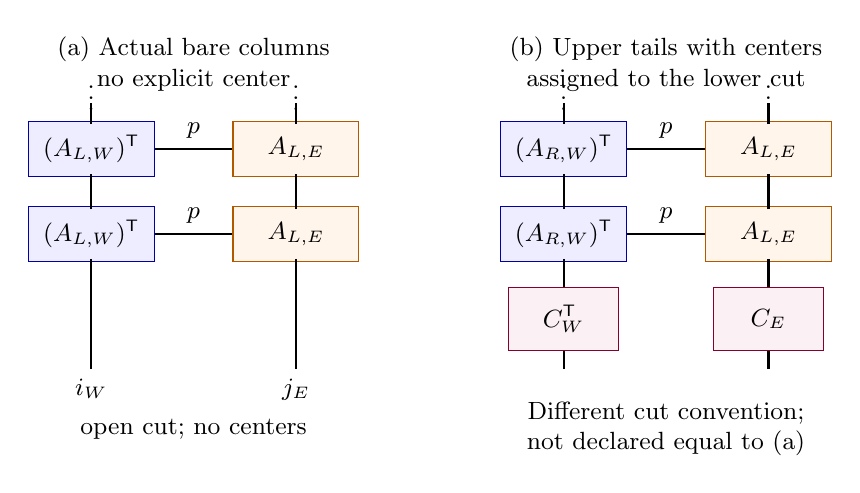
\begin{tikzpicture}[x=1cm,y=.9cm,font=\small]
\node[txt] at(1.3,4.9){(a) Actual bare columns\\no explicit center};
\node[txt] at(7.3,4.9){(b) Upper tails with centers\\assigned to the lower cut};
\foreach \y/\key in {2.5/a,3.7/b}{
 \node[m,minimum width=16mm](w\key) at(0,\y){$(A_{L,W})^{\mathsf T}$};
 \node[r,minimum width=16mm](e\key) at(2.6,\y){$A_{L,E}$};
 \draw[wire](w\key)--node[above]{$p$}(e\key);
 \node[m,minimum width=16mm](u\key) at(6,\y){$(A_{R,W})^{\mathsf T}$};
 \node[r,minimum width=16mm](v\key) at(8.6,\y){$A_{L,E}$};
 \draw[wire](u\key)--node[above]{$p$}(v\key);
}
\foreach \x in {0,2.6,6,8.6}{
 \draw[wire](\x,2.85)--(\x,3.35);
 \draw[wire](\x,4.05)--(\x,4.35);
 \node at(\x,4.53){$\vdots$};}
\draw[wire](0,2.15)--(0,.6)node[below]{$i_W$};
\draw[wire](2.6,2.15)--(2.6,.6)node[below]{$j_E$};
\node[g](cw) at(6,1.3){$C_W^{\mathsf T}$};
\node[g](ce) at(8.6,1.3){$C_E$};
\draw[wire](6,2.15)--(cw);\draw[wire](8.6,2.15)--(ce);
\draw[wire](cw.south)--(6,.6);\draw[wire](ce.south)--(8.6,.6);
\node[txt] at(1.3,-.25){open cut; no centers};
\node[txt] at(7.3,-.25){Different cut convention;\\not declared equal to (a)};
\end{tikzpicture}
\caption{Resolve the center before identifying two half-infinite networks.
Panel (a) is the actual LR input in the cardinal bare driver. Panel (b)
explicitly assigns the two centers to the cut of centered upper tails.
For LTR, insert an entire column of $a$ between the side columns, not a
single $a$ at the cut. The center-placement issue is the same.}
\label{fig:centers-at-cut}
\end{figure}

\paragraph{Moving a center changes the boundary data, not just a label.}
The exact canonical identity implies
\begin{align}
 (A_{R,W}^p)^{\mathsf T}C_W^{\mathsf T}
   &=C_W^{\mathsf T}(A_{L,W}^p)^{\mathsf T},\\
 A_{L,E}^p C_E&=C_E A_{R,E}^p.
\end{align}
Moving through $N$ sites yields
\begin{align}
 U_W^{\mathbf p}
 &=C_W^{\mathsf T}(A_{L,W}^{p_1})^{\mathsf T}\cdots
                            (A_{L,W}^{p_N})^{\mathsf T},\\
 U_E^{\mathbf p}&=C_E A_{R,E}^{p_1}\cdots A_{R,E}^{p_N}.
\end{align}
Thus one may move the west center to the \emph{far cap} while replacing
the repeated west tensors by those of the actual driver. The center has
not vanished: the far cap must be transformed. Keeping east's repeated
$A_{L,E}$ leaves its $C_E$ at the near cut; changing to repeated $A_{R,E}$
moves it to the far cap instead. In either case one must keep track of the
remaining open-bond coordinates and any inverse/support factors.

At finite depth these statements are tensor equalities with the indicated
caps. In an infinite normalized limit a changed far cap can become irrelevant
up to a scalar \emph{if} the dominant sector is unique and the cap has nonzero
overlap with it. Centers remaining at an open cut are not removed by that
argument. With degenerate sectors or singular centers, additional care is
essential. We have not established that the current $G_0=I$,
$\mathcal B_0=M_N$ and the later bare-LMPS joining implement every such
centered-tail convention. The diagram specifies the code's contraction,
not a proof that center matrices can always be dropped.

\paragraph{Source-level audit trail.}
\code{_quantum_boundary_tensor} in \code{vumps/src/quantum_sixr.jl}
exports $A_L$; \code{solve_oriented_bare_cardinal.jl} exchanges the west
bond axes and passes west/east to \code{direct_original_lmps_fixedpoints}.
That routine iterates $G$ and $\mathcal B$ without any separate $C$ input.
This is different from the endmap routine in Section~\ref{sec:endmap}, which
explicitly reads $C$ and dresses its right environment.
\fi

\begin{center}
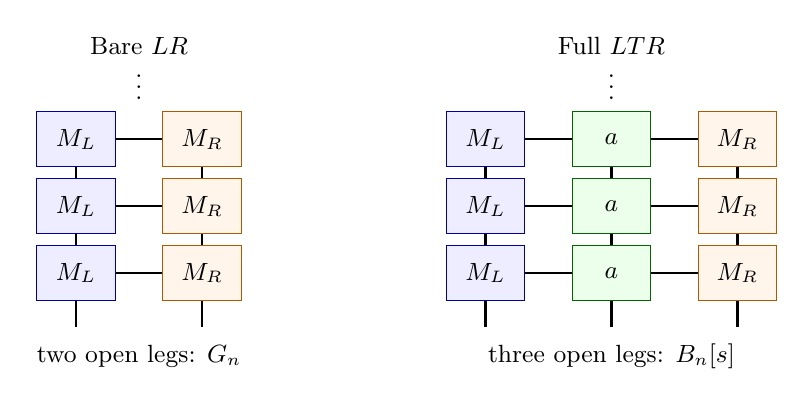
\begin{tikzpicture}[x=1cm,y=.85cm,font=\small]
\node[txt] at (0,4.4){Bare $LR$};\node[txt] at (6,4.4){Full $LTR$};
\foreach \y in {1,2,3}{
 \node[m] (l\y) at (-.8,\y){$M_L$};\node[r](r\y) at (.8,\y){$M_R$};
 \draw[wire](l\y)--(r\y);
 \node[m](b\y) at (4.4,\y){$M_L$};\node[a](a\y) at (6,\y){$a$};
 \node[r](c\y) at (7.6,\y){$M_R$};\draw[wire](b\y)--(a\y)--(c\y);
}
\foreach \x in {-.8,.8,4.4,6,7.6}{\draw[wire](\x,.2)--(\x,3.3);}
\foreach \y in {1,2,3}{
 \node[m] at (-.8,\y){$M_L$};\node[r] at (.8,\y){$M_R$};
 \node[m] at (4.4,\y){$M_L$};\node[a] at (6,\y){$a$};\node[r] at (7.6,\y){$M_R$};}
\node[txt] at (0,-.25){two open legs: $G_n$};
\node[txt] at (6,-.25){three open legs: $B_n[s]$};
\node at (0,3.9){$\vdots$};\node at (6,3.9){$\vdots$};
\end{tikzpicture}
\end{center}
Define $G_{n+1}=\mathcal E_0(G_n)$ and $B_{n+1}=\mathcal E_T(B_n)$ from specified
far caps. Their normalized limits, when they exist, define $\Gz$ and
$B_{\rm ladder}$. Every row in $B_n$ contains an $a$; it is not a single $a$
placed between bare $LR$ tails. These are exact contraction definitions for
the supplied finite-$\chi$ network. They do not remove the boundary-MPS
approximation to the original infinite PEPS.

The candidate $H^p=B_{\rm ladder}^p\Gz^+$ additionally requires compatible
sectors, relative normalization, and a specified retained support. Separate
eigen-residuals alone do not prove this candidate is the required L-shaped
network. A literal implementation is
\code{production/direct_route.jl: direct_original_lmps_fixedpoints}.

\ifdetailed
\begin{figure}[htbp]\centering
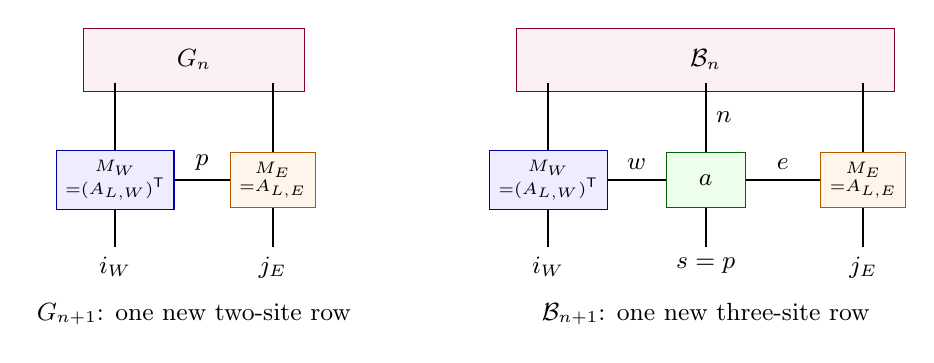
\begin{tikzpicture}[x=1cm,y=.85cm,font=\small]
\node[g,minimum width=28mm] at (1.5,2.8){$G_n$};
\node[m](ml) at (.5,1){$\substack{M_W\\=(A_{L,W})^{\mathsf T}}$};
\node[r](mr) at (2.5,1){$\substack{M_E\\=A_{L,E}}$};
\draw[wire](.5,2.45)--(ml);\draw[wire](2.5,2.45)--(mr);
\draw[wire](ml)--node[above]{$p$}(mr);
\draw[wire](ml.south)--(.5,0)node[below]{$i_W$};
\draw[wire](mr.south)--(2.5,0)node[below]{$j_E$};
\node[txt] at (1.5,-1){$G_{n+1}$: one new two-site row};
\node[g,minimum width=48mm] at (8,2.8){$\mathcal B_n$};
\node[m](wl) at (6,1){$\substack{M_W\\=(A_{L,W})^{\mathsf T}}$};
\node[a](aa) at (8,1){$a$};
\node[r](er) at (10,1){$\substack{M_E\\=A_{L,E}}$};
\draw[wire](6,2.45)--(wl);\draw[wire](8,2.45)--node[right]{$n$}(aa);
\draw[wire](10,2.45)--(er);
\draw[wire](wl)--node[above]{$w$}(aa);\draw[wire](aa)--node[above]{$e$}(er);
\draw[wire](wl.south)--(6,0)node[below]{$i_W$};
\draw[wire](aa.south)--(8,0)node[below]{$s=p$};
\draw[wire](er.south)--(10,0)node[below]{$j_E$};
\node[txt] at (8,-1){$\mathcal B_{n+1}$: one new three-site row};
\end{tikzpicture}
\caption{Literal recursion from the far end toward the open cut. The upper
box contains all previous rows of the corresponding network: $G_n$ contains
no $a$; $\mathcal B_n$ contains $n$ copies of $a$. These are not the same
tail. Here, explicitly, $M_W^p=(A_{L,W}^p)^{\mathsf T}$ and
$M_E^p=A_{L,E}^p$, from two separate VUMPS solves. Neither $C_W$ nor $C_E$
is inserted in this recursion or hidden in these boxes. Compare
Fig.~\ref{fig:centers-at-cut} for a cut-centered convention.
No rectangle endpoint is inserted.}
\end{figure}
Numerically the cardinal driver removes norm/phase growth at each step,
stores $\lambda_G,\lambda_B$, and checks both eigen-residuals. Its initial
caps are $G_0=I$ and $\mathcal B_0=M_N$. This specifies a numerical boundary
condition, not a proof of unique physical-sector selection. Store the
eigen-residuals, discarded metric rank, and strip/fidelity diagnostics.
\fi

\FloatBarrier
\subsection{Finite-depth grown-tail route: historically labelled ``direct''}
\label{sec:grown}
Absorb one local transfer tensor into one boundary tensor:
\begin{equation}\label{eq:grow}
 (\Dg^p)_{(\alpha,w),(\beta,e)}
   =\sum_n(A_L^n)_{\alpha\beta}a_{nwpe}.
\end{equation}
The enlarged bond has dimension $\chi d_{\rm eff}$; this is a local growth
step, not a contraction of an infinite column. For the mixed grown channels,
\begin{align}\label{eq:grownmaps}
 L_{n+1}^{(g)}&=\sum_p(A_L^p)^\dagger L_n^{(g)}\Dg^p,\\
 R_{n+1}^{(g)}&=\sum_p\Dg^p R_n^{(g)}(A_R^p)^\dagger.
\end{align}
Normalize with recorded scale factors. These equations have rectangular
unknowns of sizes $\chi\times\chi d_{\rm eff}$ and
$\chi d_{\rm eff}\times\chi$. At depth $n$, define
\begin{equation}\label{eq:finitegrown}
 G_n^{(g)}=L_n^{(g)}R_n^{(g)},\quad
 B_n^{(g),p}=L_n^{(g)}\Dg^pR_n^{(g)},\quad
 H_n^p=\kappa_n^{-1}B_n^{(g),p}(G_n^{(g)})^+.
\end{equation}
These are contractions of the specified \emph{grown-tail} network. They are
not a derivation of $\Gz=L_n^{(g)}R_n^{(g)}$.
The historically named TFIM direct production driver independently iterates these maps,
forms $BG^+$, and fixes its transfer normalization without reading an endpoint
checkpoint. We call this route \emph{grown-tail}; a historical CSV field
\code{method=direct} does not establish that Section~\ref{sec:bare} was used.

\ifdetailed
\begin{center}
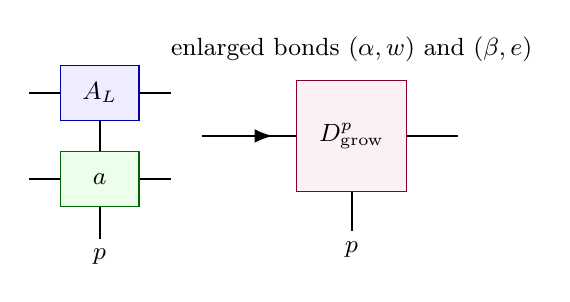
\begin{tikzpicture}[x=1cm,y=1cm,font=\small]
\node[m](m) at (0,0){$A_L$};\node[a](a) at (0,-1.1){$a$};
\draw[wire](m)--(a);
\draw[wire](m.west)--(-.9,0);\draw[wire](m.east)--(.9,0);
\draw[wire](a.west)--(-.9,-1.1);\draw[wire](a.east)--(.9,-1.1);
\draw[wire](a.south)--++(0,-.4)node[below]{$p$};
\draw[flow](1.3,-.55)--(2.2,-.55);
\node[g,minimum height=14mm](d) at (3.2,-.55){$\Dg^p$};
\draw[wire](d.west)--++(-.65,0);\draw[wire](d.east)--++(.65,0);
\draw[wire](d.south)--++(0,-.5)node[below]{$p$};
\node[txt] at (3.2,.55){enlarged bonds $(\alpha,w)$ and $(\beta,e)$};
\end{tikzpicture}
\end{center}
\begin{center}
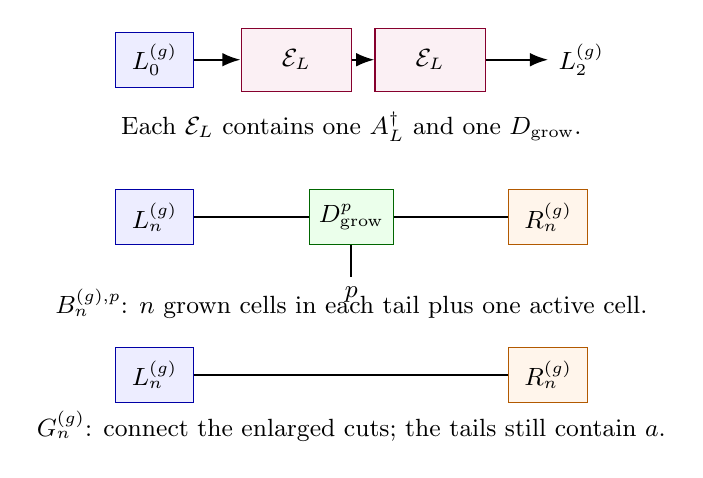
\begin{tikzpicture}[x=1cm,y=1cm,font=\small]
\node[m](l) at (0,0){$L_0^{(g)}$};
\node[g](e1) at (1.8,0){$\mathcal E_L$};\node[g](e2) at (3.5,0){$\mathcal E_L$};
\draw[flow](l)--(e1);\draw[flow](e1)--(e2);
\draw[flow](e2.east)--(5,0)node[right]{$L_2^{(g)}$};
\node[txt] at (2.5,-.85){Each $\mathcal E_L$ contains one $A_L^\dagger$ and one $\Dg$.};
\node[m](ll) at (0,-2){$L_n^{(g)}$};\node[a](dd) at (2.5,-2){$\Dg^p$};
\node[r](rr) at (5,-2){$R_n^{(g)}$};\draw[wire](ll)--(dd)--(rr);
\draw[wire](dd.south)--++(0,-.4)node[below]{$p$};
\node[txt] at (2.5,-3.1){$B_n^{(g),p}$: $n$ grown cells in each tail plus one active cell.};
\node[m](lh) at (0,-4){$L_n^{(g)}$};\node[r](rh) at (5,-4){$R_n^{(g)}$};
\draw[wire](lh)--(rh);\node[txt] at (2.5,-4.65){$G_n^{(g)}$: connect the enlarged cuts; the tails still contain $a$.};
\end{tikzpicture}
\end{center}
The factorization in Eq.~\eqref{eq:finitegrown} is exact for the finite network
just defined: it groups finite sums. It does not say that a whole half-infinite
MPS can be contracted on its own while its physical legs remain open. Those
legs are contracted against the other tensors in each mixed channel.
Likewise, replacing the tails by their converged fixed points requires a
well-defined large-depth limit, nonzero overlap with the chosen sector, and
controlled residuals. An arbitrary rectangle is not a valid environment merely
because it has the right dimensions.
\fi

\subsection{Endpoint route from VUMPS environments}
\label{sec:endmap}
For a converged boundary, the VUMPS left environment $L_{\rm env}$ is in the
$A_L$ chart and the right environment $R_{\rm env}$ is in the $A_R$ chart.
The common-chart implementation places the center explicitly:
\begin{align}
 L_{\rm end}&=L_{\rm env},&
 R_{\rm end}&=(C\otimes\id_{d_{\rm eff}})R_{\rm env},\\
 O_V&=L_{\rm end}R_{\rm end},&
 B_{\rm end}^p&=L_{\rm end}\Dg^pR_{\rm end}.
\end{align}
These are not generally the density-projector eigenvectors $V_L^\dagger,V_R$.
Using those symbols as a definition changes neither their channel nor their
proof obligations. The implementation tests the generalized relation
\begin{equation}\label{eq:bg}
 B_{\rm end}^p\simeq\kappa A_L^p O_V.
\end{equation}
On well-conditioned retained support this permits reconstruction of a local
boundary representative. Forming a pseudoinverse can amplify errors by the
metric condition number; Eq.~\eqref{eq:bg} alone cannot bound the full-array
error in $BO_V^+$. Historical canonical-completion modes reuse $A_L$ and must
not be advertised as independent tests of reconstructing it.

\ifdetailed
\paragraph{The center placement is an index statement.}
With the fused enlarged index $\mu=l+\chi(w-1)$, the symbol
$(C\otimes I)R_{\rm env}$ above means
\begin{equation}
 (R_{\rm end})_{(l,w),j}=\sum_k C_{lk}(R_{\rm env})_{(k,w),j}.
\end{equation}
This component formula, not a library-dependent Kronecker ordering, fixes
the convention. $C$ acts on the old MPS bond, not the new MPO leg $w$.

\begin{figure}[htbp]\centering
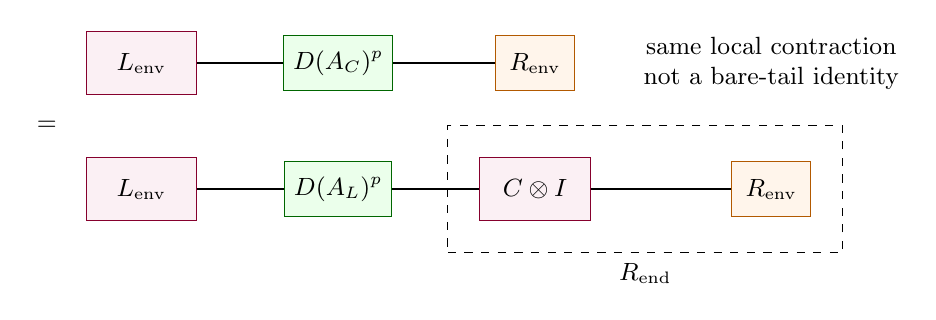
\begin{tikzpicture}[x=1cm,y=1cm,font=\small]
\node[g](le) at (0,0){$L_{\rm env}$};
\node[a](dc) at (2.5,0){$D(A_C)^p$};\node[r](re) at (5,0){$R_{\rm env}$};
\draw[wire](le)--(dc)--(re);
\node at (-1.2,-.8){$=$};
\node[g](l2) at (0,-1.6){$L_{\rm env}$};
\node[a](dl) at (2.5,-1.6){$D(A_L)^p$};
\node[g](cc) at (5,-1.6){$C\otimes I$};
\node[r](r2) at (8,-1.6){$R_{\rm env}$};
\draw[wire](l2)--(dl)--(cc)--(r2);
\node[draw,dashed,fit=(cc)(r2),inner sep=4mm,label=below:{$R_{\rm end}$}]{};
\node[txt] at (8,0){same local contraction\\not a bare-tail identity};
\end{tikzpicture}
\caption{Moving $C$ out of the active grown site onto the right environment.
This equality follows from $A_C=A_LC$ for these same tensors. It does not
identify $L_{\rm env}R_{\rm end}$ with the bare spatial $LR$ fixed point.}
\end{figure}

\paragraph{Why grown-tail and endmap can agree, and what the code does.}
After consistent center placement, compare the maps using the operators
$\mathcal F_L(X)=\sum_p(A_L^p)^\dagger X D(A_L)^p$ and
$\mathcal F_R(Y)=\sum_pD(A_L)^pY(A_R^p)^\dagger$ of Section~\ref{sec:grown}.
If both procedures solve these same operators, their dominant eigenspaces
are one-dimensional, their seeds overlap with those spaces, and all gauges
and retained supports match, their converged maps are proportional.
Writing $L_g=uL_e$, $R_g=vR_e$ then gives
$G_g=uvG_e$ and $B_g^p=uvB_e^p$: the nonzero scalar cancels in $BG^+$.
An equivalence of a full L shape further transports and normalizes both arms
and their closures consistently. Degenerate eigenspaces, different boundary
MPS solutions, finite residuals, and different support cutoffs invalidate an
unqualified equality claim.

In \code{quantum_vumps_ltr_objects}, the \emph{default}
\code{polish_endpoints=true} calls \code{direct_finite_depth_maps} with the
center-dressed VUMPS environments as initial maps. Thus this endmap path
actually refines those maps with the same grown-tail iteration. Independent
boundary solves still make it a useful reproducibility comparison, but the
tail solvers are not independent mathematical constructions. With polishing
disabled, check the raw mixed-channel residuals before making the same claim.
Neither agreement proves equivalence to the different operators
$\mathcal E_0,\mathcal E_T$ of Section~\ref{sec:bare}.
\fi

\ifdetailed
\subsection{Density projection and its approximation}
In a density-projection algorithm, a grown bond is reduced by retaining a
chosen eigenspace of a cut density matrix (or singular subspace of the
appropriate mixed contraction). In a Hermitian positive setting, if
$\rho=\sum_j w_j|j\rangle\langle j|$ with $w_j\geq0$, an isometry $V$ retains
selected columns and $VV^\dagger$ projects onto that space. The discarded
weight $\sum_{j\notin\mathrm{kept}}w_j/\tr\rho$ quantifies this particular cut's
loss; it is not, without a further argument, an error bound on $\tS$.
Left/right maps in a non-Hermitian mixed problem can be oblique, not mutual
adjoints. Their overlap must remain explicit. Choosing rectangles from a
density eigenspace is a compression prescription, whereas iterating the
grown-channel tails specifies a contraction. To identify these prescriptions,
one must show that their retained subspaces and far-boundary sectors match
and propagate correctly through the local transfer step. Citing canonical
MPS gauge identities cannot replace this demonstration.
\fi

\subsection{What equivalence would require}
A pure change of retained coordinates requires compatible maps and the
\emph{same} underlying network. For example, if invertible $U,V$ satisfy
$L'=UL$, $R'=RV$, and $B'=UBV$, then $G'=UGV$ and
$B'(G')^{-1}=U(BG^{-1})U^{-1}$. Closed contractions are unchanged when all
incident tensors are transformed consistently. This conditional algebra
does not establish its own hypotheses for two independently generated maps.

If maps insert a projector into an original cut,
\begin{equation}
 Q=R(LR)^{-1}L,\qquad
 Z-Z_Q=E_{\rm left}(\id-Q)E_{\rm right},
\end{equation}
then $Q^2=Q$ is not enough: the discarded contribution must vanish or be bounded.
For singular metrics use a declared support and recheck the support/projector
identities. No source cited here proves the unconditional identification
$\Gz=O_V$ for arbitrary quantum PEPS.

\ifdetailed
\subsection{Independence and useful numerical tests}
The independently initialized grown-tail and endpoint runs use separate seeds, boundary solves,
and intermediate checkpoints, but share the supplied PEPS and the downstream
six-$R$ implementation. Their agreement tests the compared constructions on
the tested state and tolerances, not the correctness of shared replica code.
Record finite-depth convergence, support rank, singular values, condition
numbers, $B-\kappa A_LG$ residuals, transfer spectra, mixed-boundary fidelity
where available, local observables, and finite-network contractions.
The exact RK norm free energy is an especially useful normalization check.
One matching dominant eigenvalue alone does not establish all local insertions
or all replica contractions. Finite-network regrouping and independent
CTMRG/Monte Carlo comparisons provide different checks.

\begin{center}\small
\begin{tabular}{p{35mm}p{54mm}p{54mm}}
\toprule
Route & Defining contraction & What it does not establish alone\\\midrule
Bare ladder & $\Gz=\mathrm{fp}(\mathcal E_0)$;
 $B_{\rm ladder}=\mathrm{fp}(\mathcal E_T)$ & Compatibility of $B\Gz^+$ and every L-shaped insertion.\\
Grown-tail & Explicit iteration of Eq.~\eqref{eq:grownmaps}; $G^{(g)}=L^{(g)}R^{(g)}$ & Equality of grown metric to bare metric.\\
VUMPS endpoint & Converged environments, explicit center placement, common chart & Universal exactness of finite-$\chi$ projection.\\
\bottomrule
\end{tabular}
\end{center}
\fi

\section{Oriented LMPS rails and one-copy seam metrics}
\ifdetailed
\subsection{Bare construction: which spaces belong to A and B?}
The two open bonds of $G$ and $\mathcal B[p]$ belong to the west and east
boundary frames. Record this as $G_{i_Wj_E}$ and $\mathcal B^p_{i_Wj_E}$.
Consequently $(G^+)_{j_Ek_W}$ has the opposite index order. The cardinal
implementation builds
\begin{equation}\label{eq:bare-ab}
 (H_A^p)_{i_Wk_W}=\sum_{j_E}\mathcal B^p_{i_Wj_E}(G^+)_{j_Ek_W},\qquad
 (H_B^p)_{i_Ek_E}=\sum_{j_W}(G^+)_{i_Ej_W}\mathcal B^p_{j_Wk_E}.
\end{equation}
Here $G^+$ is the declared SVD-support inverse; it is $G^{-1}$ only if full
rank is retained. Eigenvalue scales are recorded separately. $H_A,H_B$ are
not presumed canonical MPS tensors. In particular, $H_B$ is not obtained by
calling $H_A$ ``right canonical.''

\begin{figure}[htbp]\centering
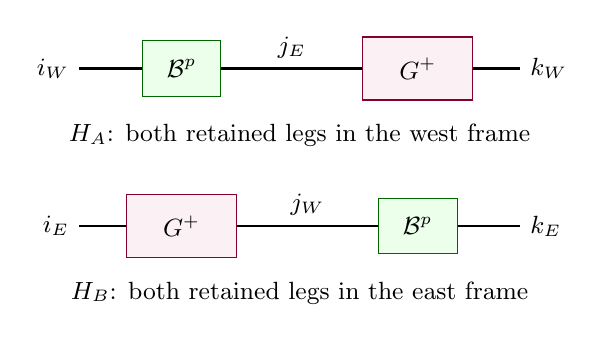
\begin{tikzpicture}[x=1cm,y=1cm,font=\small]
\node[a](ba) at (1,0){$\mathcal B^p$};\node[g](ga) at (4,0){$G^+$};
\draw[wire](-.3,0)node[left]{$i_W$}--(ba);
\draw[wire](ba)--node[above]{$j_E$}(ga);
\draw[wire](ga)--(5.3,0)node[right]{$k_W$};
\node[txt] at (2.5,-.85){$H_A$: both retained legs in the west frame};
\node[g](gb) at (1,-2){$G^+$};\node[a](bb) at (4,-2){$\mathcal B^p$};
\draw[wire](-.3,-2)node[left]{$i_E$}--(gb);
\draw[wire](gb)--node[above]{$j_W$}(bb);
\draw[wire](bb)--(5.3,-2)node[right]{$k_E$};
\node[txt] at (2.5,-2.85){$H_B$: both retained legs in the east frame};
\end{tikzpicture}
\caption{Opposite placements of the inverse metric for the two upper regions.
The labels specify array contractions, not an assumption that west and east
virtual spaces have been identified.}
\end{figure}

The rail arrays used by \code{direct_cardinal_regional_rails} are
\begin{center}\small
\begin{tabular}{lll}\toprule
Region & Horizontal ray & Vertical ray\\\midrule
$A$ & $h_A[l,p,r]=H_A[l,p,r]$ & $v_A[l,p,r]=M_W[l,p,r]$\\
$B$ & $h_B[l,p,r]=H_B[r,p,l]$ & $v_B[l,p,r]=M_E[l,p,r]$\\
$C$ & $c_L[l,p,r]=M_S[l,p,r]$, $c_R[l,p,r]=M_S[r,p,l]$ & none\\\bottomrule
\end{tabular}
\end{center}
The $M_q$ in this table have already undergone the cardinal orientation
permutations in Section~\ref{sec:bare}. Do not reflect west or south twice.

\subsection{Draw the complete bent objects before joining regions}
\begin{figure}[htbp]\centering
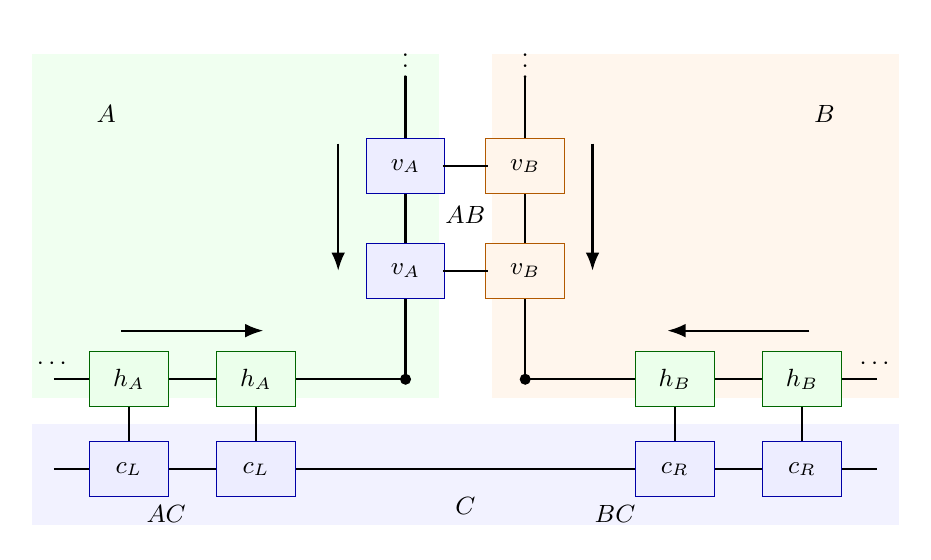
\begin{tikzpicture}[x=.95cm,y=.95cm,font=\small]
\fill[green!6](-5.8,0)rectangle(-.35,4.6);
\fill[orange!7](.35,0)rectangle(5.8,4.6);
\fill[blue!5](-5.8,-1.7)rectangle(5.8,-.35);
\node at(-4.8,3.8){$A$};\node at(4.8,3.8){$B$};\node at(0,-1.45){$C$};
\draw[wire](-5.5,.25)--(-.8,.25)--(-.8,4.3);
\draw[wire](5.5,.25)--(.8,.25)--(.8,4.3);
\foreach \x in {-4.5,-2.8}{\node[a] at(\x,.25){$h_A$};
 \draw[wire](\x,-.12)--(\x,-.6);}
\foreach \x in {2.8,4.5}{\node[a] at(\x,.25){$h_B$};
 \draw[wire](\x,-.12)--(\x,-.6);}
\foreach \y in {1.7,3.1}{\node[m] at(-.8,\y){$v_A$};
 \node[r] at(.8,\y){$v_B$};\draw[wire](-.3,\y)--(.3,\y);}
\draw[wire](-5.5,-.95)--(5.5,-.95);
\foreach \x in {-4.5,-2.8}{\node[m] at(\x,-.95){$c_L$};}
\foreach \x in {2.8,4.5}{\node[m] at(\x,-.95){$c_R$};}
\fill(-.8,.25)circle(2pt);\fill(.8,.25)circle(2pt);
\node[above] at(-5.5,.25){$\cdots$};\node[above] at(5.5,.25){$\cdots$};
\node at(-.8,4.55){$\vdots$};\node at(.8,4.55){$\vdots$};
\node at(0,2.45){$AB$};\node at(-4,-1.55){$AC$};\node at(2,-1.55){$BC$};
\draw[flow](-4.6,.9)--(-2.7,.9);\draw[flow](4.6,.9)--(2.7,.9);
\draw[flow](-1.7,3.4)--(-1.7,1.7);\draw[flow](1.7,3.4)--(1.7,1.7);
\end{tikzpicture}
\caption{Global $AB|C$ geometry. Each colored ray contains infinitely many
copies of its labelled local rail. Arrows point from the far end toward the
regional bend. The two black dots join the incident retained indices within
their own regional frame; they are not extra tensors $C_q$ or $L_{\rm end}$.
The physical links pair rails across seams. This layout is shared by the
implementations, but their rail tensors are different constructions.}
\end{figure}

To read one bent region at finite depth, give each oriented rail the array
order $[l,p,r]$, with $l$ toward the far end and $r$ toward the bend. Its
horizontal chain and vertical chain each leave one near-end index. The
implemented common-frame joining contracts those two indices. For example,
with far indices $\alpha,\beta$ left visible,
\begin{equation}\label{eq:bent-array}
 (\mathcal L_X^{(m,n)})_{\alpha\beta}^{\mathbf p,\mathbf q}
 =\sum_i(h_X^{p_1}\cdots h_X^{p_m})_{\alpha i}
         (v_X^{q_1}\cdots v_X^{q_n})_{\beta i},\quad X=A,B.
\end{equation}
This is an array-level wiring definition; no complex conjugation is implicit.
Dual legs and the physical ket/bra pairing are supplied by the scalar-network
and replica conventions. If one arm's retained basis is changed independently,
the joining tensor must change too; the displayed coordinate identity is not
a physical claim that any inter-region $K_{XY}=I$.

\smallnote{Status of the construction: the bare $G_n,\mathcal B_n$ recursions
are literal contractions of the specified networks. Choosing
Eq.~\eqref{eq:bare-ab}, these vertical rails, and the joining in
Eq.~\eqref{eq:bent-array} specifies the subsequent LMPS used in the cardinal
diagnostic. The drawing does not prove that this bent object equals every
quadrant contraction of the original PEPS. That requires compatible support,
normalization and corner/boundary conditions, and checks beyond one free
energy. The implementation preserves this distinction with
\code{production_release=false} in its reconstruction record.}

\subsection{Grown-tail/endmap rails: a different source for the vertical arms}
\fi
For endpoint/grown-tail coordinates, let $G=LR$, $R_c=RG^+$, and let $H$ be
the normalized horizontal representative. The code's array-level convention is
\begin{align}
 h_L[l,p,r]&=H[l,p,r],& h_R[l,p,r]&=H[r,p,l],\\
 v_L[l,p,r]&=L[r,l+\chi(p-1)],&
 v_R[l,p,r]&=R_c[l+\chi(p-1),r].
\end{align}
These formulas reshape and transport \emph{constructed maps}; they do not
assert $v_L=v_R=A_R$. Reflection and complex conjugation must follow the
network orientation, not an analogy with canonical labels.

\ifdetailed
In the diagram above replace $h_A,v_A$ by $A.h_L,A.v_L$, and $h_B,v_B$
by $B.h_R,B.v_R$ from these formulas. In the generic quantum path $A$ and $B$
each have a separately solved north-facing boundary and their own maps;
$C$ uses a south-facing boundary for the straight lower edge. A common chart
is constructed \emph{within} each region. This is not the cardinal bare route,
where the vertical arms come directly from $M_W,M_E$.

\begin{figure}[htbp]\centering
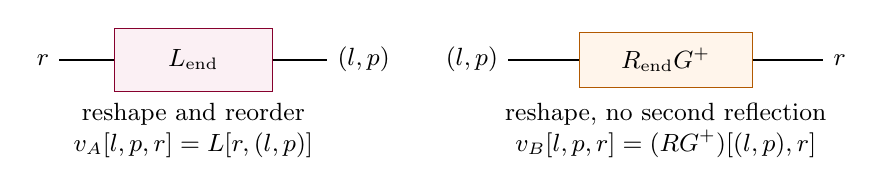
\begin{tikzpicture}[x=1cm,y=1cm,font=\small]
\node[g,minimum width=20mm](ll) at(1,0){$L_{\rm end}$};
\draw[wire](ll.west)--(-.7,0)node[left]{$r$};
\draw[wire](ll.east)--(2.7,0)node[right]{$(l,p)$};
\node[txt] at(1,-.9){reshape and reorder\\$v_A[l,p,r]=L[r,(l,p)]$};
\node[r,minimum width=22mm](rr) at(7,0){$R_{\rm end}G^+$};
\draw[wire](rr.west)--(5,0)node[left]{$(l,p)$};
\draw[wire](rr.east)--(9,0)node[right]{$r$};
\node[txt] at(7,-.9){reshape, no second reflection\\$v_B[l,p,r]=(RG^+)[(l,p),r]$};
\end{tikzpicture}
\caption{How a rectangle becomes a vertical local rail in the map-based
construction. Splitting an enlarged index is a reshape of a solved map, not
the assertion that a boundary MPS's right-canonical half equals this map.}
\end{figure}

The representative $H$ is run-dependent. The grown-tail driver's
\code{bg_pseudoinverse} mode reconstructs and normalizes $BG^+$;
\code{canonical_completion} uses the saved $A_L$ and is historical, not an
independent reconstruction check. The endmap constructor retains $A_L$ as its
stable horizontal representative and audits the reconstructed $BG^+/\kappa$.
The balanced-support option transforms $H,L,R$ together by the declared SVD
support maps. Never combine a horizontal tensor from one of these modes with
untransformed vertical rails from another.

For the real, spatially symmetric RK--Ising fast path a single boundary may
be reused after the specified spatial transformations and sector choice.
This avoids redundant solves; it does not prove bare/grown metric equality.
The frozen RK reference uses seam-local outward coordinates
(\code{production/reference_rails.jl}), rather than silently applying the
quantum global-frame map constructor. For a generic TFIM tensor do not assume
the fast path solely from the Hamiltonian's symmetry.
\subsection{Join regions using the actual mixed seam channels}
\fi

\begin{center}\small
\begin{tabular}{lll}\toprule
Seam & Incident rail in first region & Incident rail in second region\\\midrule
$AB$ & $A.v_L$ & $B.v_R$\\
$AC$ & $A.h_L$ & $C.c_L$ (or shared $h_L$)\\
$BC$ & $B.h_R$ & $C.c_R$ (or shared $h_R$)\\\bottomrule
\end{tabular}
\end{center}
For independent regions use their own rail sets. Solve the one-copy channel
\begin{equation}
 \mathcal E_{XY}^{(1)}(K_{XY})=\lambda_{XY}^{(1)}K_{XY}
\end{equation}
with physical legs paired according to the named ket/bra labels.
The resulting rank-two map connects the actual retained frames. A bare
identity is justified only after the relevant channel, orientation, support,
and coordinate identification have been demonstrated. A spatial fast path
may reuse a solved boundary; it does not set all three seam metrics to identity.

\section{Six-$R$ replica contraction}
\subsection{Permutations determine the six endpoints}
For four replicas choose
\begin{equation}
 \sigma_A=\mathrm{id},\qquad\sigma_B=(12)(34),\qquad
 \sigma_C=(13)(24).
\end{equation}
Region $X$ pairs ket copy $i$ with bra copy $\sigma_X(i)$.
The relative permutations across the seams give
\begin{equation}
 AB: (12),(34);\quad AC:(13),(24);\quad BC:(14),(23).
\end{equation}
Each cycle supplies a rank-four endpoint $\mathcal R_{XY,ij}$ with retained
legs $(X,i),(X,j),(Y,i),(Y,j)$ and the corresponding explicit bra labels.
Thus the six objects are $AB12,AB34,AC13,AC24,BC14,BC23$.
They are not six unrelated GS calculations, and they need not be equal arrays
even when a single C4v boundary was reused.

\ifdetailed
\begin{center}
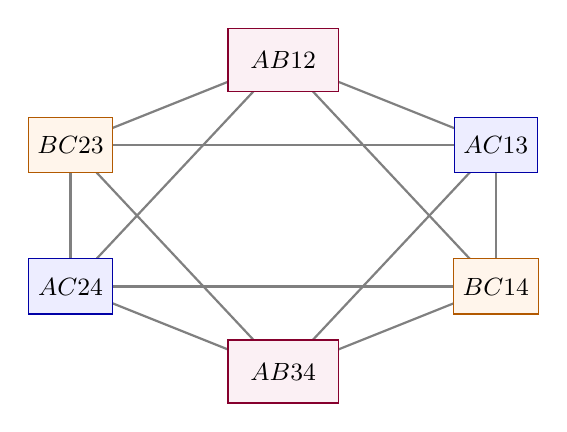
\begin{tikzpicture}[scale=.9,every node/.style={font=\small}]
\coordinate (u) at (0,2.2);\coordinate(d)at(0,-2.2);
\coordinate(v)at(3,1);\coordinate(w)at(3,-1);
\coordinate(x)at(-3,-1);\coordinate(y)at(-3,1);
\foreach \a/\b in {u/v,u/x,u/w,u/y,d/v,d/x,d/w,d/y,v/w,v/y,x/w,x/y}
 {\draw[gray,thick](\a)--(\b);}
\node[g]at(u){$AB12$};\node[g]at(d){$AB34$};
\node[m]at(v){$AC13$};\node[m]at(x){$AC24$};
\node[r]at(w){$BC14$};\node[r]at(y){$BC23$};
\end{tikzpicture}
\end{center}
\smallnote{Octahedral connectivity of $Z_4$: every logical edge $(X,i)$ occurs
on exactly two endpoints. Crossings in this drawing are not additional vertices.}

\subsection{Fixed-point direction and physical far-boundary amplitude}
For each replica seam, solve right and left eigenproblems
\begin{equation}
 \mathcal E_{XY,ij}(\mathcal R)=\lambda\mathcal R,
 \qquad \mathcal E_{XY,ij}^{\dagger}(\mathcal L)
       =\overline\lambda\mathcal L.
\end{equation}
The finite physical tail is $F_n=\mathcal E^n(F_0)$. For a simple dominant
eigenvalue and nonzero overlaps,
\begin{equation}
 F_n\sim\lambda^n\mathcal R\,
 \frac{\langle\mathcal L,F_0\rangle}{\langle\mathcal L,\mathcal R\rangle}.
\end{equation}
Normalizing $\mathcal R$ to unit norm discards the coefficient unless it is
tracked separately. Construct the replica cap from the one-copy physical seam
caps with the correct permutation and retain its scalar prefactor. The current
code checks eigen-residuals, left/right consistency, far-cap alignment, and
the convergence of the log-amplitude after removing the extensive eigenvalue.
Near degeneracy the displayed single-eigenvector asymptotic may fail or converge
slowly. A small residual does not guarantee that the physical far cap selects
that eigenvector. Do not release an entropy just because an eigensolver stopped.
\fi

\subsection{Closing $Z_1,Z_{2X},Z_4$ and forming the observable}
Contract all six endpoints on their twelve shared regional/copy edges to form
$Z_4$. The untwisted $Z_1$ uses the three one-copy seam maps. Each ordinary
two-replica sector reuses two of the six rank-four endpoints and closes its
remaining identity cycle with the appropriate rank-two map:
\begin{center}\small
\begin{tabular}{lll}\toprule
Sector & Rank-four endpoints reused & Untwisted seam\\\midrule
$Z_{2A}$ & $AB12,AC13$ & $BC$\\
$Z_{2B}$ & $AB34,BC14$ & $AC$\\
$Z_{2C}$ & $AC24,BC23$ & $AB$\\\bottomrule
\end{tabular}
\end{center}
It is not a bare trace of two rank-four tensors. With compatible finite-network
normalization, define
\begin{align}
 S_2(X)&=-\ln(Z_{2X}/Z_1^2),&
 S_2^{(3)}&=-\tfrac12\ln(Z_4/Z_1^4),\\
 \tS&=2S_2^{(3)}-S_2(A)-S_2(B)-S_2(C)
      =-\ln\frac{Z_4Z_1^2}{Z_{2A}Z_{2B}Z_{2C}}.\label{eq:stilde}
\end{align}
For infinite seams, use the synchronized constant terms after removing length
growth. Each endpoint's arbitrary rescaling must cancel with its exact
multiplicity in Eq.~\eqref{eq:stilde}. The implementation tests this explicitly.
Complex phases must also be audited: a code-level $\ln|Z|$ is not permission
to discard an unexplained phase of a purported physical partition function.

\ifdetailed
\subsection{Why plotted components can be negative}
Production tables additionally use a straight-half-plane reference. Let
$I_1,I_4,I_{2X}$ denote the synchronized log-intercepts, including far-boundary
prefactors. The local-window components are
\begin{align}
 S_{2A}^{\rm loc}&=-(I_{2A}-I_{2C}),&
 S_{2B}^{\rm loc}&=-(I_{2B}-I_{2C}),& S_{2C}^{\rm loc}&=0,\\
 S_3^{\rm loc}&=-\tfrac12(I_4+2I_1-3I_{2C}).
\end{align}
They are reference-subtracted constants, not positive density-matrix entropies.
Their combination is the same $\tS$. Store both raw and local conventions;
labels such as ``S3'' in a CSV must state which is used. In particular $S_3$
here is a tripartite replica quantity, not the ordinary R\'enyi entropy of order
three. A dip in $\tS$ may arise from cancellation between its components.
Sharing the same $\mathcal R$ library does not force all these combinations
to have the same sensitivity to errors.

\subsection{Contraction cost and checks independent of the maps}
The named-edge topology must be audited before evaluating numerical tensors.
Contract each logical edge exactly once; moving a junction tensor into a rail
does not authorize inserting it again in the final closure. Large octahedron
intermediates may be evaluated by exact index slicing: sum every slice and
compare with unsliced contractions at small sizes. Slicing changes memory and
time, not the represented network; discarding slices would be an additional
approximation. One-copy, two-copy and four-copy normalizations must remain
synchronized through such changes.
\fi

\section{Correlation lengths, critical fields, and convergence}
For a transfer step of physical length $\ell$,
\begin{equation}
 \xi=-\ell/\ln|\lambda_1/\lambda_0|.
\end{equation}
State which transfer matrix, direction, eigenvalue sector and blocking length
define the plotted $\xi$. A boundary-MPS self-transfer length, a physical
connected-spin length, and a CTMRG transfer estimate are not automatically
identical. A cat-state near-degeneracy can encode long-range order rather than
the connected correlator's decay. Hence no universal prescription doubles
every broken-state boundary length.

\ifdetailed
For the axis-direction square-lattice Ising spin correlator, define the dual
coupling $\beta^*=-\tfrac12\ln\tanh\beta$ and the elementary mass
$m_1=2|\beta^*-\beta|$. The disordered spin exponential length is $1/m_1$;
on the ordered side the connected spin correlation has exponential length
$1/(2m_1)$. These are asymptotic decay lengths, not a second-moment length.
Near criticality $m_1\sim4|\beta-\beta_c|$, with
$\beta_c=\tfrac12\ln(1+\sqrt2)$. Any comparison must specify this phase and
observable convention, rather than call $1/[2|\beta-\beta_c|]$ the exact
spin length. The RK state norm provides the classical Ising reference;
critical wavefunction entanglement and geometric contributions are discussed
in Ref.~\cite{fradkin}, not a proof of a particular fitted $\tS$ coefficient.
\fi

At fixed saved PEPS $A_D(h)$, scan $\chi$ without reoptimizing that PEPS.
Saturation of $\xi(\chi)$ is compatible with a finite-correlation-length
finite-$D$ state even near the physical TFIM transition; see
Refs.~\cite{rader,corboz}. A critical RK tensor can instead remain critical
at fixed finite PEPS $D$. Thus a log-$\chi$ trend in RK--Ising does not require
the same trend for every optimized finite-$D$ TFIM tensor.

To locate a finite-$D$ pseudocritical region, inspect $\xi(h)$ on a dense grid
at several environment/boundary dimensions, together with branch energies and
magnetizations. Bracket the peak; do not call the largest sampled point an
exact critical field. Plot $\xi$ versus $\chi$, $\tS$ versus $\chi$, and
$\tS$ versus the \emph{same run's} $\xi$ in three aligned rows. Report source
hashes and missing/failed points. Fit a logarithm or power law only in a
demonstrated window, with fit-range and convergence uncertainties.

\section{Reproducibility and evidence status}
The normative numerical records are saved tensors, source hashes, method
identifiers, solver tolerances, residuals, and replica components, not a PNG
or a successful Slurm exit code. A pair can contain two individually accepted
measurements and still disagree. Keep such pairs visible as unresolved.
Neither numerical route agreement nor a passed symmetry check is a theorem
about arbitrary quantum states. No universal $\tS\sim\ln\chi$ coefficient or
complete all-$D$ convergence is claimed in this methods note.

\ifdetailed
\subsection{Implementation map}
Paths below are relative to \code{code2d/lmps/}.
\begin{description}
\item[State preparation.] \code{core/ising.jl};
\code{vumps/src/quantum.jl}; production GS drivers in \code{vumps/benchmarks/}.
\item[Boundary VUMPS.] \code{vumps/src/boundary.jl} and quantum boundary routines
in \code{vumps/src/quantum.jl}. Retain TensorKit leg orientations.
\item[Bare ladders and finite-depth grown maps.]
\code{production/direct_route.jl}; distinguish
\code{direct_original_lmps_fixedpoints} from \code{direct_finite_depth_maps}.
\item[Cardinal bare diagnostic (Section 4.1).]
\code{vumps/benchmarks/solve_oriented_bare_cardinal.jl};
\code{direct_cardinal_regional_rails} in \code{production/direct_route.jl};
\code{vumps/benchmarks/quantum_tfim_bare_ladder_sixr_diagnostic.jl}.
\item[Historically named direct production (grown-tail, Section 4.2).]
\code{vumps/production/quantum_tfim_direct_scan_point.jl};
\code{bg_pseudoinverse} and independently initialized boundaries.
\item[Endpoint production.]
\code{vumps/src/quantum_sixr.jl};
\code{vumps/production/quantum_tfim_common_chart_scan_point.jl} and
its \code{best_boundary} variant have different candidate-selection rules.
\item[Geometry and replica closure.]
\code{core/sixr.jl} specifies descriptors and wiring;
\code{core/sixr_closure.jl} constructs rails, solves seams and forms ratios.
\item[Validation.] Source-specific audits under \code{vumps/benchmarks/};
pair checks under \code{vumps/plots/}. Inspect pair status in addition to
individual convergence. Capture code and dependency-manifest hashes per run.
\end{description}

\subsection{Minimal record for one measured point}
Record $(\mathrm{model},D,h\text{ or }\beta,\chi_{\rm CTM},\chi)$, GS hash and
parent, symmetry/sector convention, method version, random seeds, candidate
selection, metric rank/condition, environment and replica residuals, far-cap
amplitude tests, $\xi$ convention, all $S_2/S_3$ components, and $\tS$.
Store the raw six-$R$ checkpoints separately from compact tables and plots.
Use Slurm for numerical computation, tests, compilation and rendering.
The organized results directory is a curated access layer; live jobs retain
their established paths until a checked migration can be performed.
\fi

\begin{thebibliography}{9}
\bibitem{vumps} V. Zauner-Stauber, L. Vanderstraeten, M. T. Fishman,
F. Verstraete, and J. Haegeman, ``Variational optimization algorithms for
uniform matrix product states,'' Phys. Rev. B \textbf{97}, 045145 (2018).
\href{https://arxiv.org/abs/1701.07035}{arXiv:1701.07035}.
\bibitem{schollwock} U. Schollw\"ock, ``The density-matrix renormalization group
in the age of matrix product states,'' Ann. Phys. \textbf{326}, 96--192 (2011).
\href{https://arxiv.org/abs/1008.3477}{arXiv:1008.3477}.
\bibitem{ctm} T. Nishino and K. Okunishi, ``Corner Transfer Matrix
Renormalization Group Method,'' J. Phys. Soc. Jpn. \textbf{65}, 891--894 (1996).
\href{https://arxiv.org/abs/cond-mat/9507087}{arXiv:cond-mat/9507087}.
\bibitem{liao} H.-J. Liao, J.-G. Liu, L. Wang, and T. Xiang,
``Differentiable Programming Tensor Networks,'' Phys. Rev. X \textbf{9},
031041 (2019). \href{https://arxiv.org/abs/1903.09650}{arXiv:1903.09650}.
\bibitem{rader} M. Rader and A. M. L\"auchli, ``Finite Correlation Length
Scaling in Lorentz-Invariant Gapless iPEPS Wave Functions,'' Phys. Rev. X
\textbf{8}, 031030 (2018).
\href{https://arxiv.org/abs/1803.08566}{arXiv:1803.08566}.
\bibitem{corboz} P. Corboz, P. Czarnik, G. Kapteijns, and L. Tagliacozzo,
``Finite correlation length scaling with infinite projected entangled-pair
states,'' Phys. Rev. X \textbf{8}, 031031 (2018).
\href{https://arxiv.org/abs/1803.08445}{arXiv:1803.08445}.
\bibitem{fradkin} E. Fradkin and J. E. Moore, ``Entanglement entropy of 2D
conformal quantum critical points: hearing the shape of a quantum drum,''
Phys. Rev. Lett. \textbf{97}, 050404 (2006).
\href{https://arxiv.org/abs/cond-mat/0605683}{arXiv:cond-mat/0605683}.
\end{thebibliography}
\end{document}
